\section{Experiments}
In this section, we briefly present our experiments on some of the 
algorithms presented at the previous sections. Two sets of experiments are presented.

The first tests are on powers
of random gaussian matrices of different sizes. The goal of this set of numerics
is to check the performance of the algorithms and make sure they are working
as expected. We also analyze the sharpness of the bounds dictated by the theory.
In particular, the bound on the expectation of the error given
by \ref{thm:avg-frob-error-gauss} and
the error estimation procedure which was motivated by 
Lemma \ref{thm:aposteriori}.
We have used an \textit{oversampling parameter} $p=5$ for all of the experiments.

The second set of experiments analyses the performance of the
\textit{Randomized Power Method} \ref{alg:randomized-power-iteration} on MNIST
and on a matrix appearing in image processing.

\subsection{Details of the implementation}
The experiments have been implemented in \verb|Matlab|. The reproducible
source code can be found at the following 
\href{https://github.com/alexnowakvila/ProbAlgosProj}{Github repository}
together with the \LaTeX~  of the report. Please read \verb|README| documentation
to run the code on the \verb|Matlab| interactive command line.
\subsection{Gaussian Matrices} \label{sec:gaussian-matrices}
In this set of experiments, we test and analyze the performance of the 
Algorithms \ref{alg:randomized-range-finder}, 
\ref{alg:adaptive-randomized-range-finder},
\ref{alg:randomized-power-iteration}
and \ref{alg:fast-randomized-range-finder}.

The experiments are performed on powers of gaussian random
matrices of the form:

\begin{equation}\label{eq:gaussian-matrices}
\mtx{A} = \frac{1}{\sqrt{m}+\sqrt{n}}\mtx{G}, \hspace{0.5cm}
 G_{ij}\sim N(0,1)
\end{equation}
The normalization in \ref{eq:gaussian-matrices} is to make sure that the norm
of $\mtx{A}$ is around 1 with high probability
\footnote{This is a direct consequence of Sudakov-Fernique's inequality that
compares the supremum of two gaussian processes when one is dominated
by the other. More precisely, you have the bound on the expectation
of the norm $\Expect\|\mtx{G}\|\leq\sqrt{m}+\sqrt{n}$
and also an accompanying tail bound 
$\Prob{\|\mtx{G}\| \geq \sqrt{m} + \sqrt{n} + t}\leq 2\exp(-ct^2)$.
Using Gordon's inequality (generalization of Sudakov Fernique's), you can
also prove lower bounds on the smallest singular value
$\Expect\|\mtx{G}^\dagger\|\geq \sqrt{m} - \sqrt{n}$ and
$\Prob{\|\mtx{G}\|\leq \sqrt{m}-\sqrt{n}-t}\leq 2\exp(-ct^2)$.
These results on concentration of measure have been studied at the Theory
Reading Group following the book on High Dimensional Probability
from R.Vershynin which I highly recommend 
\cite{vershynin2016high}.}.
As seen from Equation \ref{eq:sing-values-power}, the singular values decay faster 
for higher powers of the matrix.
\subsubsection{Experiments on Randomized Range Finder 
\ref{alg:randomized-range-finder}} See Figure \ref{fig:exp1-1}.
\begin{figure}[H]\label{fig:exp1-1}
\begin{center}
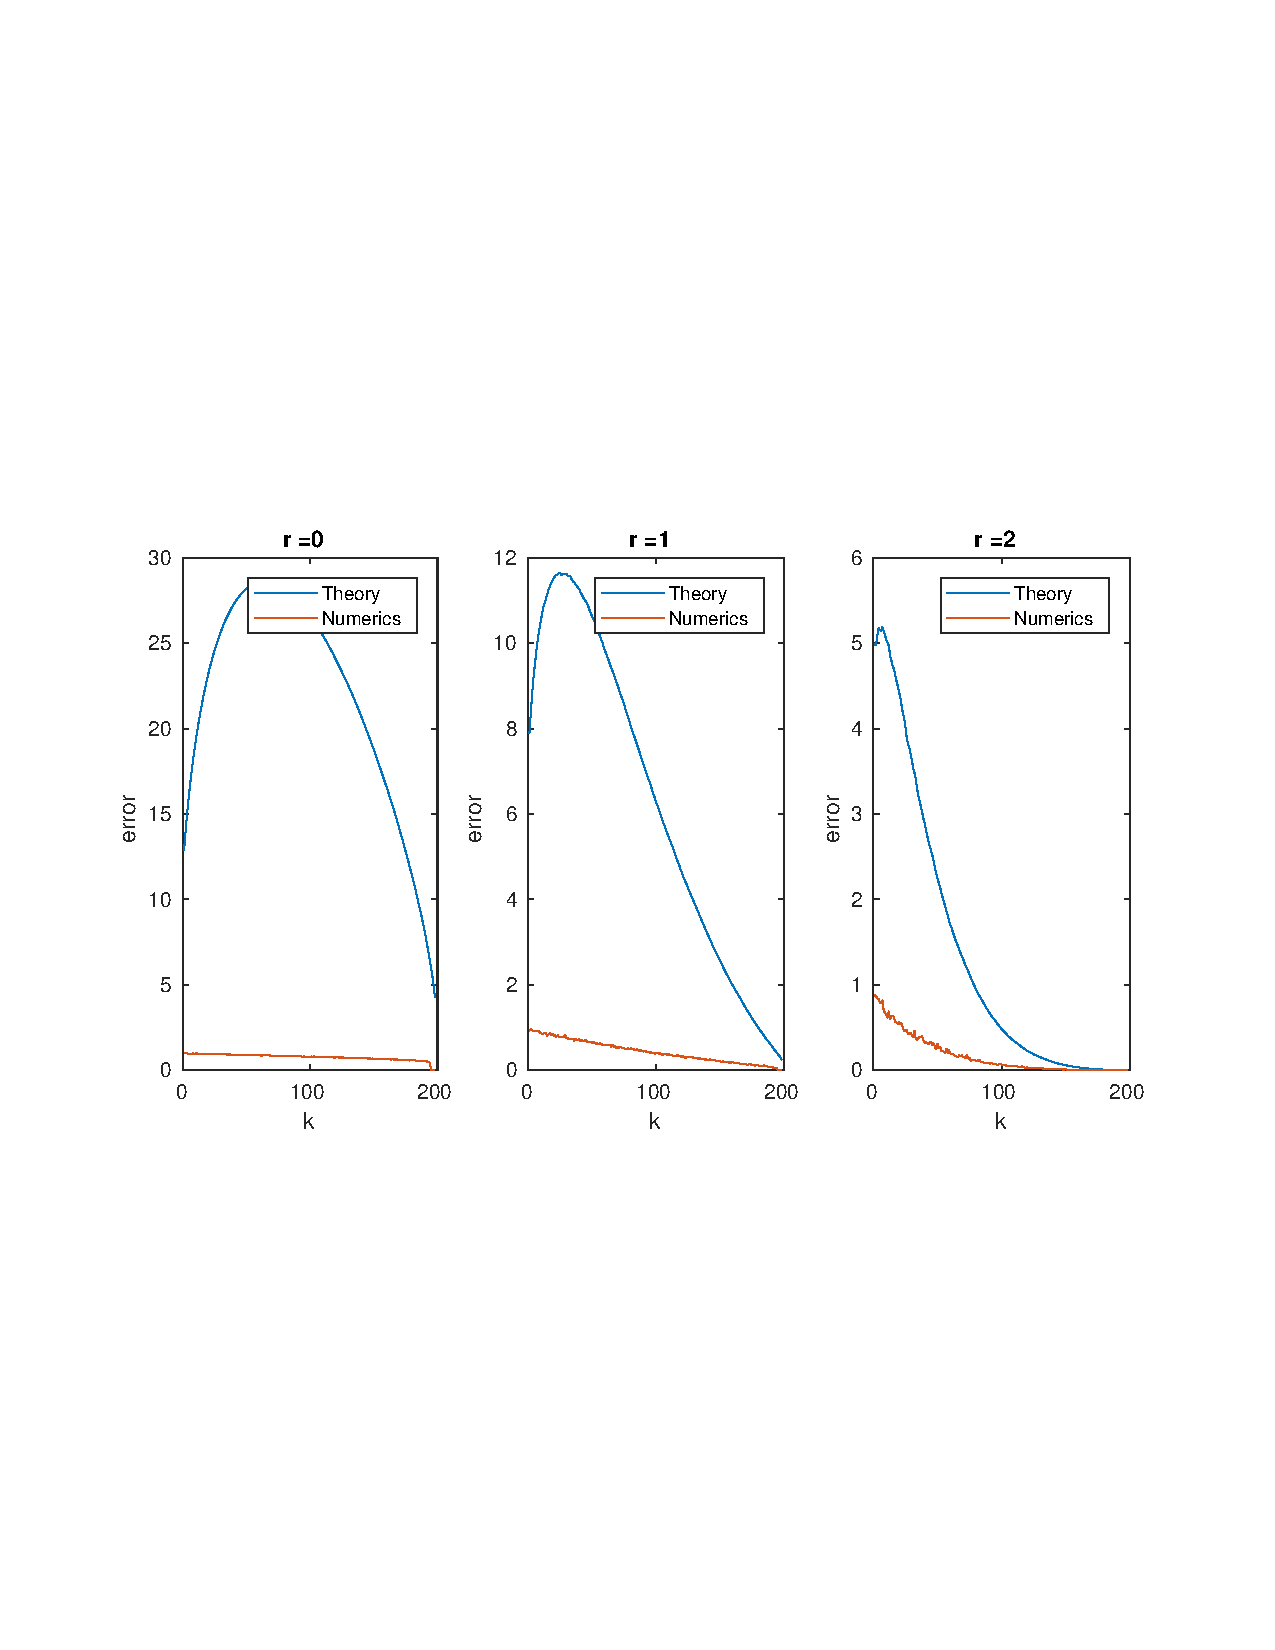
\includegraphics[width=\textwidth, trim=0cm 8cm 0cm 9cm, clip=true]{figures/1-4.pdf}
\end{center}
\caption{Comparison between theoretical mean bound \ref{thm:avg-frob-error-gauss}
and numerical error \ref{eq:range-error} produced by Algorithm \ref{alg:randomized-range-finder}
 for $(\mtx{A}\mtx{A}^\adj)^r\mtx{A}$ with $r=0,1,2$. }
\end{figure}

\subsubsection{Experiments on Randomized Power Iteration 
\ref{alg:randomized-power-iteration}} See Figure \ref{fig:exp1-2}.
\begin{figure}[H] \label{fig:exp1-2}
\begin{center}
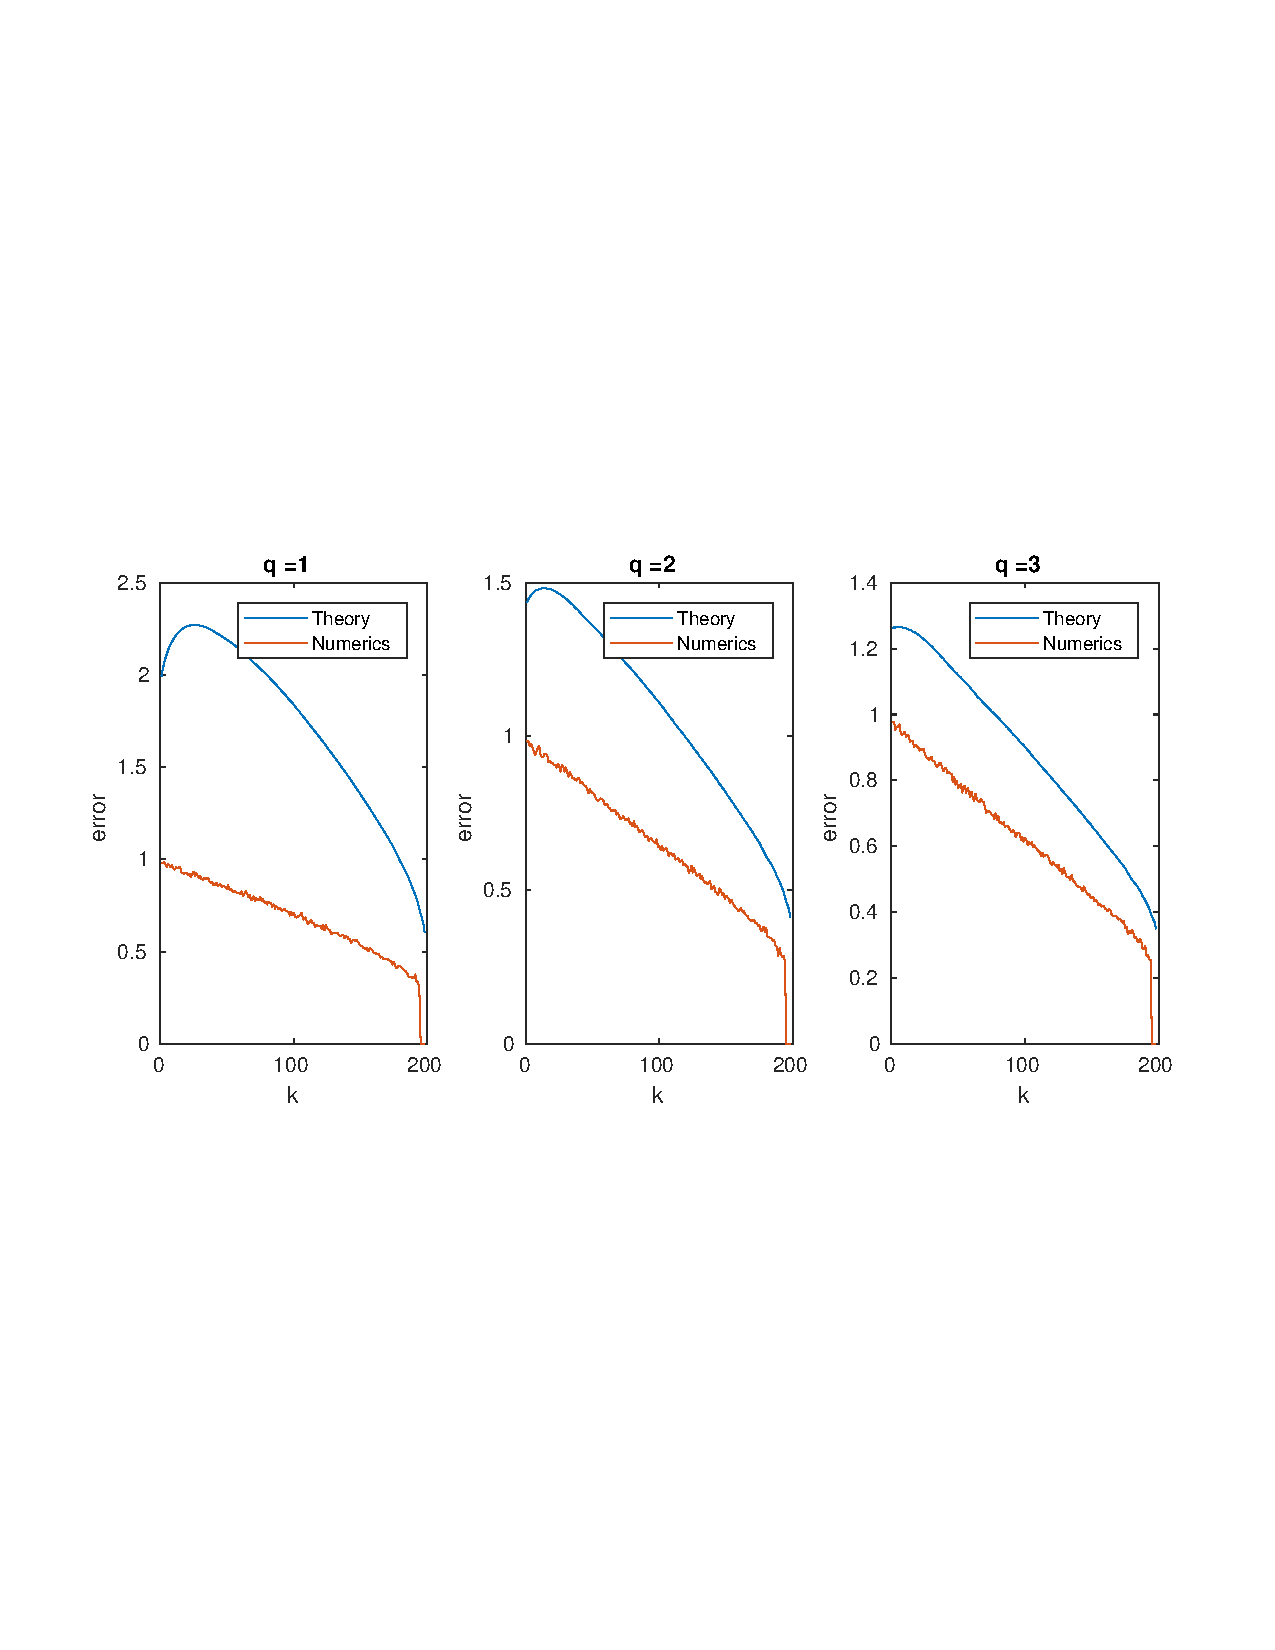
\includegraphics[width=\textwidth, trim=0cm 8cm 0cm 9cm, clip=true]{figures/1-5.pdf}
\end{center}
\caption{Comparison between theoretical mean bound from Corollary
\ref{cor:power-method-spec-gauss} and numerical
error \ref{eq:range-error} produced by Algorithm \ref{alg:adaptive-randomized-range-finder}
for $\mtx{A}$ and $q=1,2,3$}
\end{figure}

\subsubsection{Experiments on Adaptive Randomized Range Finder
\ref{alg:adaptive-randomized-range-finder}}
In this experiment, Algorithm \ref{alg:adaptive-randomized-range-finder} is applied
to $(\mtx{A}\mtx{A}^\adj)^2\mtx{A}$ with pre-specified tolerances ranging
from 0 to 1. We have fitted a line to the numerical
error produced vs the tolerance (the dependence was close to linear). The slope of the
resulting line
is $\textbf{0.045}$, i.e, for the matrices used in the experiment, the 
bound \ref{eq:errorest} has a numerical suboptimality of 0.045.
\subsubsection{Experiments on Fast Randomized Range Finder
\ref{alg:fast-randomized-range-finder}}
Algorithm \ref{alg:fast-randomized-range-finder} has been applied to several
powers of $\mtx{A}$ (using SRFT test matrices) and the error curve for 
different target ranks is essentially the same as the one found using
Algorithm \ref{alg:randomized-range-finder}.

\subsection{Real Datasets}
\subsubsection{MNIST}
In this experiment, we used 10,000 examples from
the MNIST dataset \cite{lecun1998mnist} of 28x28
black and white images of handwritten digits.

The goal is to compare Algorithm \ref{alg:randomized-range-finder} with the
power version \ref{alg:randomized-power-iteration} on the matrix
$\mtx{M}\in\Rspace{10000\times 784}$ where each row is a flattened image.
The singular values of $\mtx{M}$ decay fast, hence, the power scheme does not
significantly improve the randomized scheme for $q>1$.
See Figure \ref{fig:exp2}.

\subsubsection{A Large, Sparse, Noisy Matrix Arising in Image Processing}
One way to tackle standard tasks in image processing is to use the information
about the local geometry of the image through the \textit{graph Laplacian}.
The dominant eigenvectors of this operator provide coordinates that help to smooth
out noisy image patches \cite{szlam2008regularization}.

First, define $\widetilde{\mtx{W}}$ as
\begin{equation}\label{eq:similarities}
\widetilde{w}_{ij}=\exp\{-\|\mtx{x}^{(i)} - \mtx{x}^{(j)}\|^2/\sigma^2\}
\end{equation}
where $\mtx{x}^{(i)}$ is a vector gathering the intensities of a neighborhood
of a certain size of the pixel $i$. Here, $\sigma$ controls the level of
sensitivity. We then define the sparse matrix $\mtx{W}$ constructed by
zeroing out all the entries in $\widetilde{\mtx{W}}$ except the 7 largest
ones in each row. 
Finally, the laplacian operator is defined as
\begin{equation}\label{eq:graph-laplacian}
\mtx{L}=\mtx{I}-\mtx{D}^{-1/2}\mtx{W}\mtx{D}^{-1/2}
\end{equation}
where $\mtx{D}$ is the diagonal matrix with entries $d_{ii}=\sum_{j}w_{ij}$.

In order to find the low-frequency eigenvectors of $\mtx{L}$,
we must find the eigenvectors with dominant eigenvalues of

\begin{equation}\label{eq:adj}
\mtx{A}=\mtx{D}^{-1/2}\mtx{W}\mtx{D}^{-1/2}
\end{equation}

In our experiment, we have taken a patch of size 57x57 from the classical
$\verb|Lenna.png|$ photo. The matrix $\widetilde{\mtx{W}}$ is constructed 
with patches of size 5x5 centered at the corresponding pixel with
zero-padding at the boundary. The resulting
matrix $\mtx{A}$ has size 3249x3249 and has low decaying eigenvalues. Hence,
as can be seen in Figure \ref{fig:exp2}, the power scheme from
Algorithm \ref{alg:randomized-power-iteration} is very advantageous.

\begin{figure}[H] \label{fig:exp2}
\begin{center}
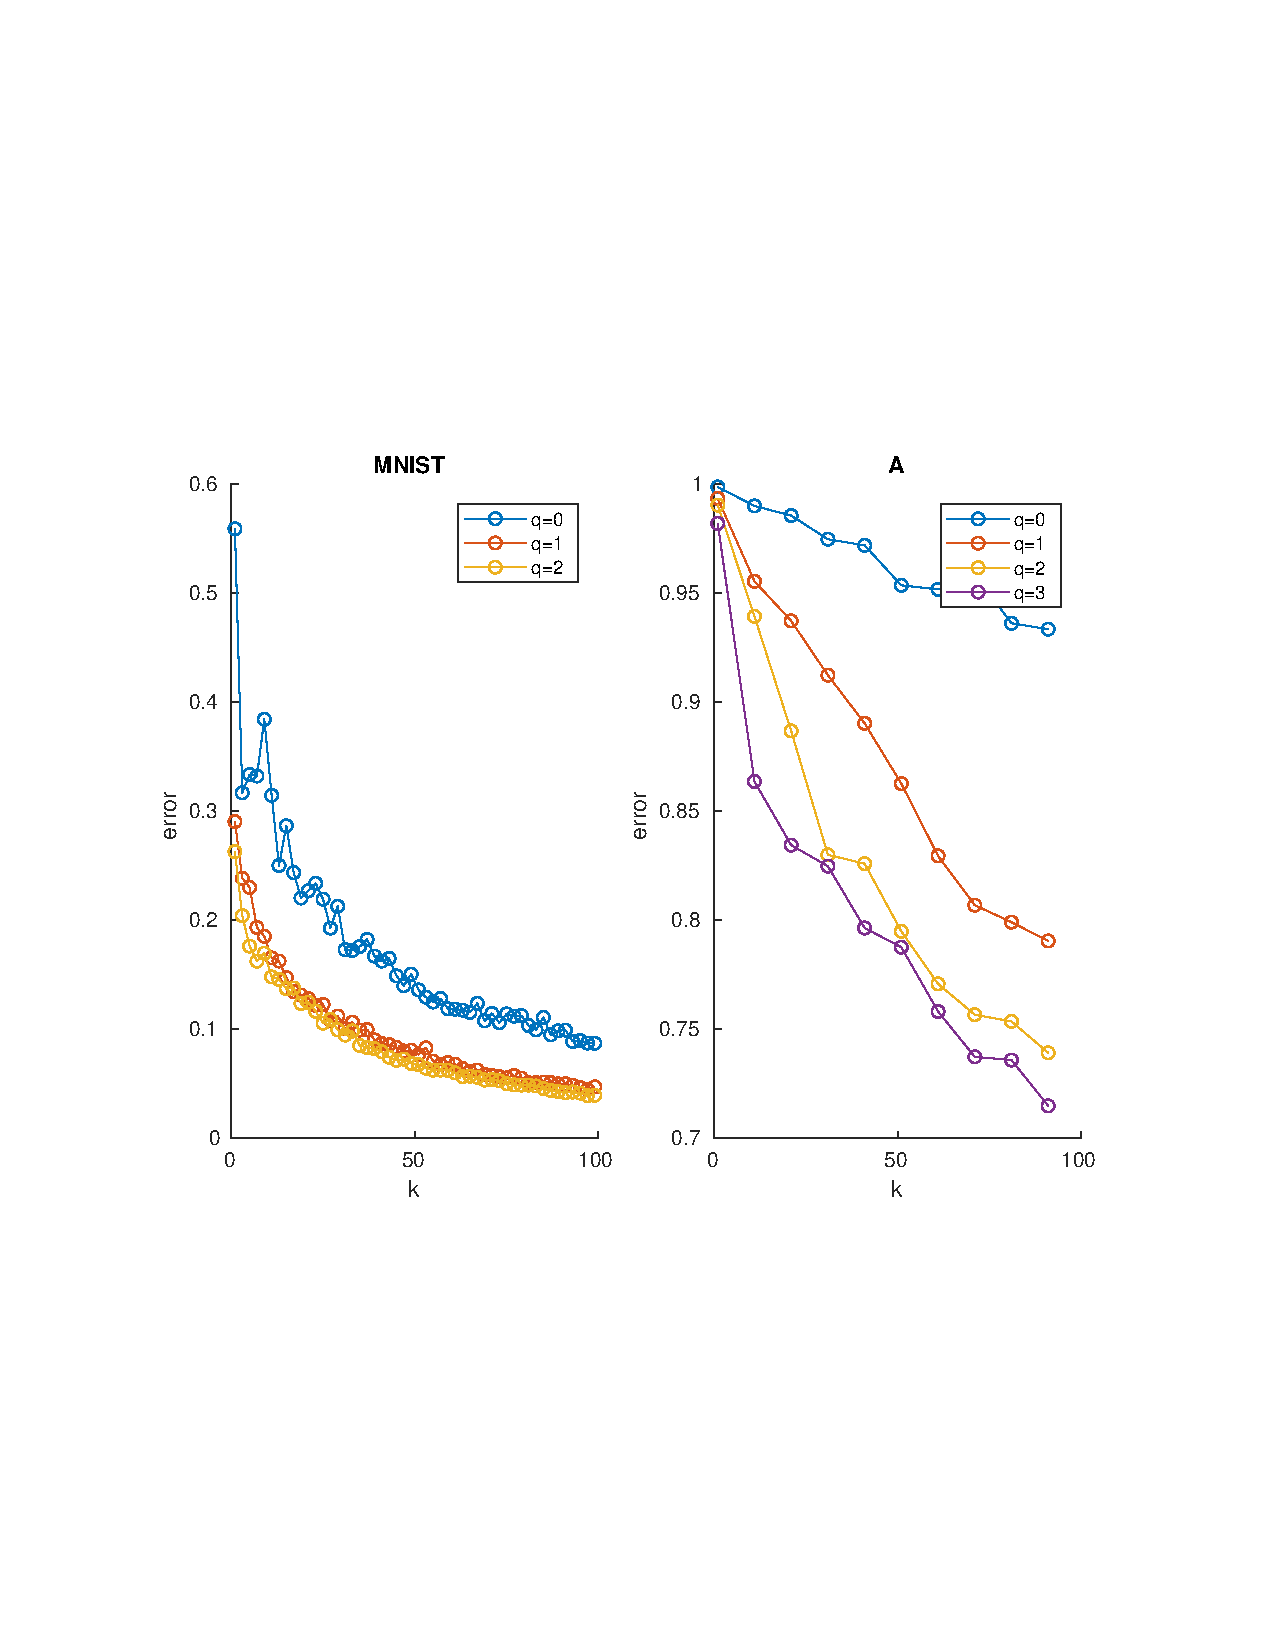
\includegraphics[width=\textwidth, trim=0cm 8cm 0cm 7cm, clip=true]{figures/2-2.pdf}
\end{center}
\caption{Approximation error \ref{eq:range-error} for the
power scheme \ref{alg:randomized-power-iteration} for MNIST 
(Left) and $\mtx{A}$ \ref{eq:adj} (Right) for $k$ ranging from $1$ to $100$.}
\end{figure}